\chapter{Implementation}

\label{chap:Implem}


In this chapter the core functionalities of the card sorting capabilities of
Diamond are presented. Most importantly, the actual sorting implementation is 
explained. Furthermore, all other aspects, such as creating a card sort study
or exporting and possible analytics of the results are also discussed.


\section{Creating a Card Sort}

The main structure of card sort study creation was taken from the previously 
implemented TreeTest, but it was not copied entirely. Adjustments were made to
better represent a card sort study. 

Every study has a name and an option to include a mandatory password to guard
the study from unwanted participants. Then a welcome message, instructions as
well as a thank you message and feedback message can be specified. These
messages are customizable to facilitate easy adjustments according to the needs
of the respective study.

Cards can be added manually through an input text field. After creation there is
also the possibility of renaming or deleting previously added cards. Another way
of loading the wanted cards is by importing the dataset via a .csv file. Here 
any number of cards, separated by a comma or semicolon, are included into the
study card list for later sorting. Note that using the import function clears
any previously added cards, as this helps unintentionally mixing datasets.

A screenshot of the card sort creation can be viewed in
Figure~\ref{fig:creation}. 


\begin{figure}[tp]  \centering
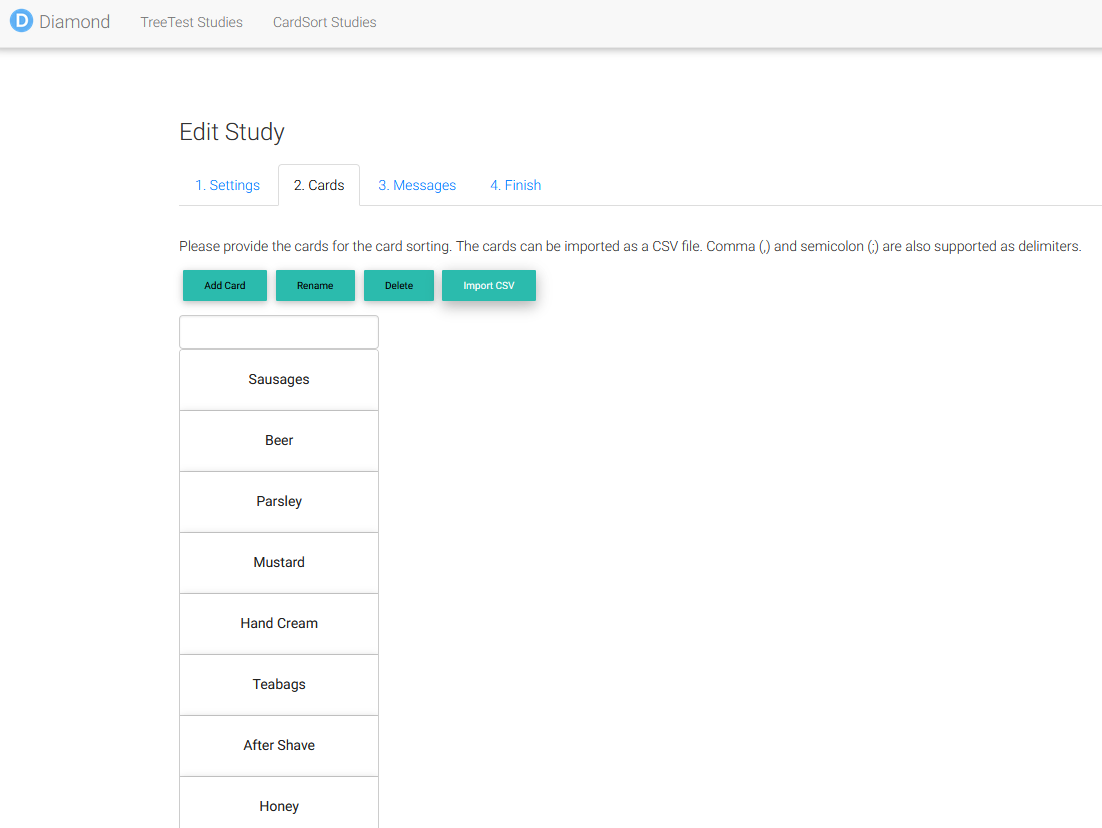
\includegraphics[keepaspectratio,width=\linewidth,height=\halfh]{images/implementation/create.png}
\caption[Card Sort Study Creation] 
{The graphical user interface during the adding of cards to a card sort study.
\imgcredit{Screenshot was captured by Christopher Oser using
Diamond.} } 
\label{fig:creation} 
\end{figure}

\section{Taking part in a Study}

Once a card sort study has been created, it is possible to share it to users.
This can be done via a link and possibly a password to further control the users
taking part in the study. Each user needs to specify their name and receives
the previously defined welcome message and instructions before attempting the
actual sorting.

The card sorting itself is made up of the card list, which is presented to the
user on the left of the screen, and a dedicated area for groups that are to be
defined by the user. The cards in the card list are stacked vertically and the
remaining amount of cards in the list can be seen at the very top.  

Currently Diamond only supports open card sorting, which, according to Prof.
Keith Andrews, ``..is the only true form of card sorting''. Therefore all groups
need to be defined by the user. This can be done via a input text field. Once a
group is added, cards can be dragged from the card list to a group of choice.
All groups can be renamed or deleted. Did a deleted group contain cards, these
cards are then added back to the card list to be sorted again. A screenshot of
the card sorting process can be viewed in Figure~\ref{fig:sorting}.

\begin{figure}[tp]  \centering
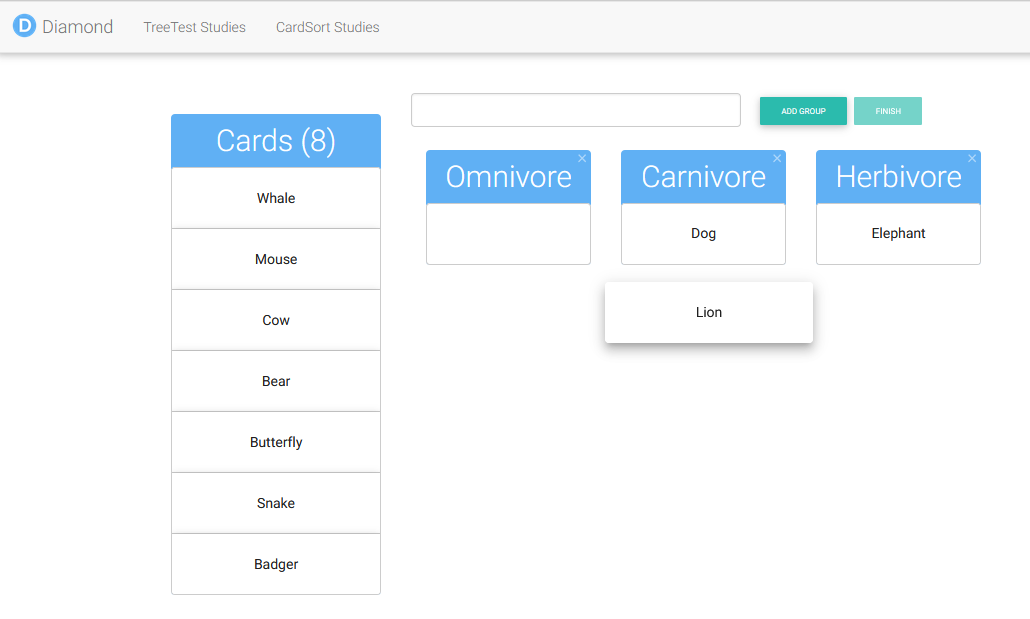
\includegraphics[keepaspectratio,width=\linewidth,height=\halfh]{images/implementation/sorting.png}
\caption[Card Sorting Interface] 
{The graphical user interface during the sorting of cards by the user.
\imgcredit{Screenshot was captured by Christopher Oser using
Diamond.} } 
\label{fig:sorting} 
\end{figure}

Once all cards have been assigned to groups the user has the option to finish
their sort. The next step for the user is to explain their mindset during the
sorting, to facilitate better analytics of the results. After this, the user is
presented with the option to provide general feedback concerning the study.

\section{Evaluating Results}

At any point during the study, the study manager, the person who created the
study, can view and export the results of the study. The results are composed by
the name of the user, the date of the sorting, the sorting results, the mindset
and the feedback message. The general overview of the results of a study can be
viewed in Figure~\ref{fig:results}. The sorting results are displayed on a
separate page for each user, they are made up by a table where each column
represents one group. A sample table can be viewed in Figure~\ref{fig:table}.

The results can also be exported for later use in .csv format. There are two
different files that are ready for export. The first is the user data, comprised
by names, dates, feedback messages and mindsets. The data is represented per row
per user. The second file is the sorting data over all users. Here the data is
represented by all cards in the first row, followed by a one user per row group
assignment to the respective card in the column. So each user's sorting data is
represented by a row of groups.

\begin{figure}[tp]  \centering
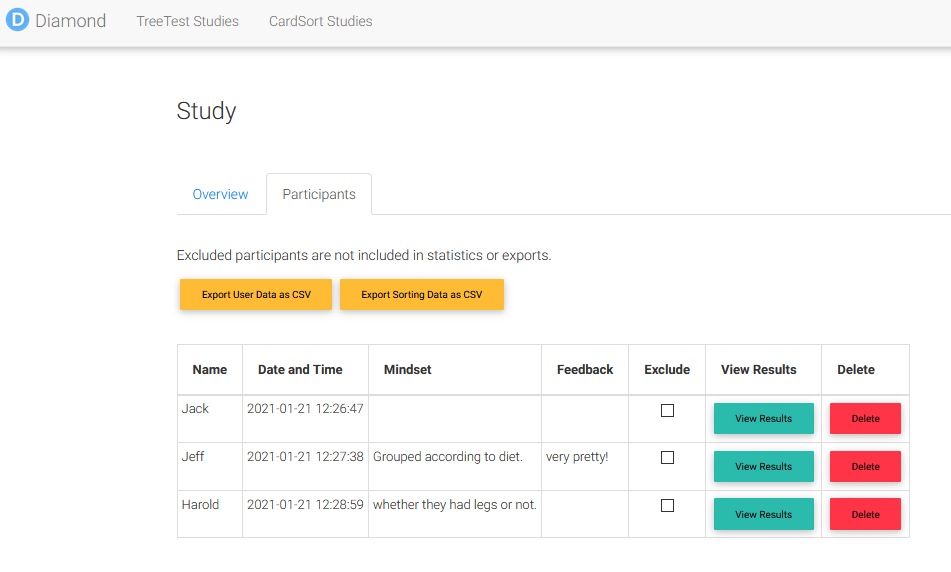
\includegraphics[keepaspectratio,width=\linewidth,height=\halfh]{images/implementation/results.png}
\caption[Card Sorting Results Overview] 
{The overview over the results of a card sort study in Diamond.
\imgcredit{Screenshot was captured by Christopher Oser using
Diamond.} } 
\label{fig:results} 
\end{figure}

\begin{figure}[tp]  \centering
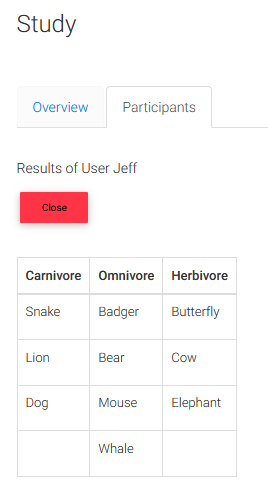
\includegraphics[keepaspectratio,width=\linewidth,height=\halfh]{images/implementation/table.png}
\caption[Card Sorting Result Table] 
{The table that represents the sorting results of one user. Each group is represented
by a column and the respective cards are listed below the first row.
\imgcredit{Screenshot was captured by Christopher Oser using
Diamond.} } 
\label{fig:table} 
\end{figure}